\section{同変Schubert計算}
\subsection{Grassmann多様体の同変コホモロジー}
$\text{Gr}_k(\complex^n)=\set{V\subset \complex^n}{\dim V = k}$をGrassmann多様体という.$T=\complex^n$とするとき,$T$は$\complex^n$に
\[
(t_1,\cdots,t_n)\cdot(x_1,\cdots,x_n)=(t_1x_1,\cdots,t_nx_n)
\]
によって左から作用する.この作用は自然に$\text{Gr}_k(\complex^n)$への作用を誘導し,$\text{Gr}_k(\complex^n)$は$T$空間となる.$\text{Gr}_k(\complex^n)$の$T$同変コホモロジーの構造は組み合わせ的に決定することができる.
$\binom{n}{k}$を$0$と$1$からなる$n$文字の文字列のうち,$1$が$k$個使われている文字列の集合とする.$\lambda=\lambda_1\cdots \lambda_n\in\binom{n}{k}$に対して置換$\sigma\in\mathfrak{S}_n$の$\binom{n}{k}$への作用を$\sigma\lambda=\lambda_{\inv{\sigma}(1)}\cdots\lambda_{\inv{\sigma}(n)}$で定める.
$\lambda=\lambda_1\cdots \lambda_n\in\binom{n}{k}$に対して,
\[
\Omega_\lambda^\circ=\set{V\in \text{Gr}_k(\complex^n)}{\dim(V\cap F_i)= \dim(\complex^{\lambda}\cap F_i),\quad \forall i\in \{1,\cdots n\}}
\]
をSchubert cellという.ここで,$\complex^{\lambda}=\langle\lambda_{1}e_{1},\cdots,\lambda_ne_n\rangle$, $F_i=\langle e_{1},\cdots,e_i\rangle$である. 

\begin{prop}
  $\text{inv}(\lambda)=\set{(i,j)}{\lambda_i=1, \lambda_j=0, i<j}$とすると$\Omega_\lambda^\circ$は$\complex^{\binom{n}{k}-|\text{inv}(\lambda)|}$に同相であり
\begin{equation}\label{CW str of grassmannian}
\text{Gr}_k(\complex^n)=\bigsqcup_{\lambda\in\binom{n}{k}}\Omega_\lambda^\circ
\end{equation}
 となる.またこれによって$\text{Gr}_k(\complex^n)$はCW-複体の構造をもつ.
\end{prop}

\begin{proof}
  $M(k,n)$をランク$k$の$k\times n$複素行列全体のなす集合とする.$\text{GL}_k(\complex)$は自然に$M(k, n)$に左作用するが$\text{Gr}_k(\complex^n)$は自然に$M(k,n)/\text{GL}_k(\complex)$と同一視される.$\lambda$を左から読んで$1\leq i_1<\cdots<i_k\leq n$番目に$1$が現れるとする.
  このとき$\Omega_\lambda^\circ$は
  \small
  \begin{equation}\label{row echelon form}
  \left(\begin{array}{ccc}
    {\begin{array}{ccccccccccc}
    * & \cdots & * & \overbrace{1}^{i_1\text{-th column}} & 0 & \cdots & 0 & \overbrace{0}^{i_{2}\text{-th column}} & 0 & \cdots & 0\\
    * & \cdots & * & 0 & * & \cdots & * & 1 & 0 & \cdots & 0\\
    \vdots & \ddots & \vdots & \vdots & \vdots & \ddots & \vdots & \vdots & \vdots & \ddots & \vdots\\
    * & \cdots & * & 0 & * & \cdots & * & 0 & * & \cdots & * 
    \end{array}} & \cdots & 
    {\begin{array}{ccccccc}
    0 & \cdots & 0 & \overbrace{0}^{i_{k}\text{-th column}} & 0 &\cdots & 0\\
    \vdots & \ddots & \vdots & \vdots & \vdots & \ddots & \vdots\\
    0 & \cdots & 0 & 0 & 0 & \cdots & 0\\
    * & \cdots & * & 1 & 0 & \cdots & 0
    \end{array}}
  \end{array}\right)
\end{equation}
  \normalsize
  この形の行列で代表される$M(k,n)/\text{GL}_k(\complex)$の点の集合と同一視できる.ここで$*$は任意の複素数である.また,各cellは$T$不変であることもわかる.

  次に(\ref{CW str of grassmannian})が$\text{Gr}_k(\complex^n)$のCW構造となることを示す.$E_\lambda\subset M(k, n)$を
  \small
  \begin{equation}\label{orthonormal form}
  \left(\begin{array}{ccc}
    {\begin{array}{ccccccccccc}
    * & \cdots & * & \overbrace{x_1}^{i_1\text{-th column}} & 0 & \cdots & 0 & \overbrace{0}^{i_{2}\text{-th column}} & 0 & \cdots & 0\\
    * & \cdots & * & * & * & \cdots & * & x_2 & 0 & \cdots & 0\\
    \vdots & \ddots & \vdots & \vdots & \vdots & \ddots & \vdots & \vdots & \vdots & \ddots & \vdots\\
    * & \cdots & * & * & * & \cdots & * & * & * & \cdots & * 
    \end{array}} & \cdots & 
    {\begin{array}{ccccccc}
    0 & \cdots & 0 & \overbrace{0}^{i_{k}\text{-th column}} & 0 &\cdots & 0\\
    \vdots & \ddots & \vdots & \vdots & \vdots & \ddots & \vdots\\
    0 & \cdots & 0 & 0 & 0 & \cdots & 0\\
    * & \cdots & * & x_k & 0 & \cdots & 0
    \end{array}}
  \end{array}\right)
\end{equation}
\normalsize
  この形の行列のなす集合とする.ここで,$x_i\geq 0$であり,行ベクトルは正規直交であるとする.
  
  $E_\lambda$がclosed ballに同相であることを示す.$H_{a}=\set{(z_1,\cdots,z_{a},0,\cdots,0)\in\complex^n}{\sum|z_j|^2=1,z_{a}\geq 0}$とする.$\pi\colon E_\lambda\rightarrow H_{i_1}$を$1$行目を取り出す写像とし,
  $v=(0,\cdots,0,\overbrace{1}^{i_1\text{-th}},0,\cdots,0)$とおく.このとき$E_\lambda\approx H_{i_1}\times\inv{\pi}(v)$が成り立つ.さらに$\lambda'\in\binom{n-1}{k-1}$を$i_2-1,\cdots,i_k-1$番目に$1$が現れる文字列とすると$\inv{\pi}(v)=E_{\lambda'}$であるから
  \[
  E_\lambda\approx H_{i_1}\times E_{\lambda'}
  \]
  となる.よって帰納的に$E_\lambda$がclosed ballに同相であるとわかる.

  自然な写像$\varphi\colon E_\lambda\rightarrow\text{Gr}_k(\complex^n)$によって$E_\lambda^\circ$は$\Omega_\lambda^\circ$に写されるが,$\varphi\colon E_\lambda^\circ\rightarrow\Omega_\lambda^\circ$は全単射であるから同相である.また$\varphi(\partial E_\lambda)\subset \bigcup_{\mu < \lambda} \Omega_{\mu}^\circ$であることも明らか.ただし$\mu \leq \lambda \Leftrightarrow \sum_{i=1}^j\mu_i \leq \sum_{i=1}^j \lambda_i$である.
\end{proof}

$\overline{\Omega_\lambda^\circ}$は既約な多様体となることが知られており,$H^*(\text{Gr}_k(\complex))$は$\overline{\Omega_\lambda^\circ}$の定めるホモロジー類$[\overline{\Omega}_\lambda]$のPoincare双対$\sigma_\lambda$たちで$\integer$上生成される\cite{fulton young tableaux}.

$T$空間$X$に対して$H^*_T(X)$は$ET\times_TX$のコホモロジーであったが,$ET$は有限次元近似$ET_r$を持っている(§1.1).$\overline{\Omega_\lambda^\circ}$は$T$不変であるから,$ET_r\times_T\overline{\Omega_\lambda^\circ}$は$H^*(ET_r\times_T\text{Gr}_k(\complex^n))$においてホモロジー類$[\overline{\Omega}_\lambda]$を定める.このPoincare双対$\sigma_\lambda$の極限によって$H^*_T(\text{Gr}_k(\complex^n))$の元が定まる.これをSchubert classといい,$S_\lambda$とおく(?).

$\text{Gr}_k(\complex^n)$はequivariantly formalであるから同型
$H^*_T(\text{Gr}_k(\complex^n))\simeq H^*(\text{Gr}_k(\complex^n))\otimes H^*_T(\text{pt})$が存在する.$S_\lambda\in H^*(ET\times_T\text{Gr}_k(\complex))$は各ファイバーに制限すると$\sigma_\lambda$に一致するから
\[
S_\lambda = \sigma_\lambda + \sum_{I}c_Iy^I
\]
と展開できる.ここで$c_I\in H^*(\text{Gr}_k(\complex^n))$の次数は$|\lambda|$より小さい.よって帰納的に$\sigma_\lambda$が$\{S_\lambda\}_\lambda$の線形結合で表せることがわかるので,$\{S_\lambda\}_\lambda$は$H^*T(\text{Gr}_k(\complex^n))$の基底となる.


$2$つのSchubert classの積$S_\lambda S_\mu$を$\{S_\nu\}_{\nu\in\binom{n}{k}}$の$\integer[y_1,\cdots,y_n]$係数の線形結合で
\begin{equation}\label{LRcoeff}
  S_\lambda S_\mu=\sum_{\nu\in\binom{n}{k}}C^\nu_{\lambda\mu}S_\nu
\end{equation}
このように表したとき,係数$C^{\nu}_{\lambda\mu}$を計算する組み合わせ的手法を紹介することが本論文の目的である.





\subsection{GKM条件によるSchubert Classの特徴づけ}

$\text{Gr}_k(\complex^n)$の$T$作用における固定点は$\{\complex^\lambda\}_{\lambda\in\binom{n}{k}}$であるから,[GKM]より$H^*_T(\text{Gr}_k(\complex^n))$は$\bigoplus_{\lambda\in\binom{n}{k}}H^*_T(\text{pt})$の部分代数である.GKMの定理を適用するために$\text{Gr}_k(\complex^n)$の$T$不変な$\mathbb{CP}^1$を計算する.

\begin{prop}
  $\lambda,\mu\in\binom{n}{k}$に対して$\complex^\lambda$と$\complex^\mu$を結ぶ$T$不変な$\mathbb{CP}^1$が存在するための必要十分条件は,ある$(i, j)\in\text{inv}(\lambda)$に対して$\mu = (i, j)\lambda$
  となっていることである.
\end{prop}

\begin{proof}
  $\lambda\in\binom{n}{k}$, $\mu=(i, j)\lambda$ (for $(i,j)\in\text{inv}(\lambda))$に対して,$\phi\colon \mathbb{CP}^1\rightarrow \text{Gr}_k(\complex^n)$を
  \[
  \phi([x:y])=
  \left(
  \begin{array}{}
    0 & \cdots & 0 & 1 & 0 & \cdots
  \end{array}
  \right)
  \]
\end{proof}

次に


[GKM]より
\[
H^*_T(\text{Gr}_k(\complex^n))=\set{(f_\lambda)_{\lambda\in\binom{n}{k}}\in\bigoplus_{\lambda\in\binom{n}{k}}H^*_T(\text{pt})}{f_\lambda-f_{\lambda'}}
\]







\subsection{Schubert puzzleによる方法}

\begin{defin}
  以下の$8$種類のラベル付きの図形をpuzzle pieceと呼ぶ.
  \begin{center}
    \begin{tikzpicture}
      \coordinate (A) at (0,0);
      \coordinate (B) at (2,0);
      \coordinate (C) at (1,1.7);

      \draw (A)--(B)--(C)--cycle;
      \node[font=\large] at ($(A)+(1,-0.25)$) {$0$};
      \node[font=\large] at ($(A)+(0.3,1)$) {$0$};
      \node[font=\large] at ($(A)+(1.7,1)$) {$0$};

      \coordinate(P) at (3,0);
      \draw ($(A)+(P)$)--($(B)+(P)$)--($(C)+(P)$)--cycle;
      \node[font=\large] at ($(P)+(1,-0.25)$) {$1$};
      \node[font=\large] at ($(P)+(0.3,1)$) {$1$};
      \node[font=\large] at ($(P)+(1.7,1)$) {$1$};

      \coordinate (Q) at (6,0);
      \draw ($(A)+(Q)+(0,1.7)$)--($(B)+(Q)+(0,1.7)$)--($(C)+(Q)-(0,1.7)$)--cycle;
      \node[font=\large] at ($(Q)+(0.2,0.8)$) {$0$};
      \node[font=\large] at ($(Q)+(1.8,0.8)$) {$0$};
      \node[font=\large] at ($(Q)+(1,2)$) {$0$};

      \coordinate (R) at (9,0);
      \draw ($(A)+(R)+(0,1.7)$)--($(B)+(R)+(0,1.7)$)--($(C)+(R)-(0,1.7)$)--cycle;
      \node[font=\large] at ($(R)+(0.2,0.8)$) {$1$};
      \node[font=\large] at ($(R)+(1.8,0.8)$) {$1$};
      \node[font=\large] at ($(R)+(1,2)$) {$1$};

      \draw ($(A)-(0,3)$)--($(B)-(0,3)$)--($(C)-(0,3)$)--($(C)-(2,3)$)--cycle; 
      \node[font=\large] at ($(A)+(1,-3.25)$) {$0$};
      \node[font=\large] at ($(A)+(1.8,-2.2)$) {$1$};
      \node[font=\large] at ($(A)+(-0.8,-2.2)$) {$1$};
      \node[font=\large] at ($(A)+(0,-1)$) {$0$};

      \draw ($(A)-(-3,3)$)--($(B)-(-3,3)$)--($(C)-(-5,3)$)--($(C)-(-3,3)$)--cycle;
      \node[font=\large] at ($(P)+(1,-3.25)$) {$1$};
      \node[font=\large] at ($(P)+(2.9,-2)$) {$0$};
      \node[font=\large] at ($(P)+(0.3,-2)$) {$0$};
      \node[font=\large] at ($(P)+(2,-1)$) {$1$}; 

      \draw ($(A)+(6.5,-2.5)$)--($(C)+(6.5,-2.5)$)--($(B)+(6.5,-2.5)$)--($(C)+(6.5,-5.9)$)--cycle;
      \node[font=\large] at ($(Q)+(0.8,-1.5)$) {$1$};
      \node[font=\large] at ($(Q)+(2.2,-1.5)$) {$0$};
      \node[font=\large] at ($(Q)+(2.2,-3.5)$) {$1$};
      \node[font=\large] at ($(Q)+(0.8,-3.5)$) {$0$};

      \fill[cyan] ($(A)+(9.5,-2.5)$)--($(C)+(9.5,-2.5)$)--($(B)+(9.5,-2.5)$)--($(C)+(9.5,-5.9)$)--cycle;
      \draw[thick] ($(A)+(9.5,-2.5)$)--($(C)+(9.5,-2.5)$)--($(B)+(9.5,-2.5)$)--($(C)+(9.5,-5.9)$)--cycle;
      \node[font=\large] at ($(R)+(0.8,-1.5)$) {$0$};
      \node[font=\large] at ($(R)+(2.2,-1.5)$) {$1$};
      \node[font=\large] at ($(R)+(2.2,-3.5)$) {$0$};
      \node[font=\large] at ($(R)+(0.8,-3.5)$) {$1$};
    \end{tikzpicture}
  \end{center}
  ただし,puzzle pieceのうち三角形のものは$1$辺の長さが$1$の正三角形であり,平行四辺形のものは$1$辺の長さが$1$で鋭角は$60$度であるとする.またpuzzle pieceのうち
    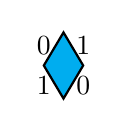
\begin{tikzpicture}[baseline=-1pt]
      \fill[cyan] (0,0)--(0.25,0.42)--(0.5,0)--(0.25,-0.42)--cycle;
      \draw[thick] (0,0)--(0.25,0.42)--(0.5,0)--(0.25,-0.42)--cycle;
      \node at (0,0.25) {$0$};
      \node at (0.5,0.25) {$1$};
      \node at (0,-0.25) {$1$};
      \node at (0.5,-0.25) {$0$};
    \end{tikzpicture}
  をequivariant pieceという.
\end{defin}

\begin{defin}
  いくつかのpuzzle pieceを(同一種のpieceは何個用いてもよい)同じラベルを持つ辺に沿って貼り合わせ,一つの大きな正三角形を作ったものをpuzzleと呼ぶ.puzzle $P$を上向きの正三角形となるように見たとき,$P$の左上の辺上に存在するラベルたちを下から上に読んで得られる文字列を$\lambda$,$P$の右上の辺上に存在するラベルたちを上から下に読んで得られる文字列を$\mu$,下の辺上に存在するラベルたちを左から右に読んで得られる文字列を$\nu$とする.このとき
  \[
  \partial P = \Delta^{\nu}_{\lambda\mu}
  \]
  と書く.
\end{defin}

\begin{eg}
  $\partial P=\Delta^{1010}_{0110,1001}$をみたすpuzzleは

  \begin{center}
    \begin{tikzpicture}
      \draw (0,0)--(8,0)--(4,6.8)--cycle;
      \draw (2,0)--(3,1.7)--(1,1.7);
      \draw (3,1.7)--(4,0)--(5,1.7)--(6,0);
      \draw (5,1.7)--(7,1.7);

      \draw (2,3.4)--(3,1.7)--(4,3.4)--(5,1.7)--(6,3.4);
      \draw (2,3.4)--(6,3.4);

      \draw[thick] (3,5.1)--(4,3.4)--(5,5.1)--(4,6.8)--cycle;
      \fill[cyan] (3,5.1)--(4,3.4)--(5,5.1)--(4,6.8)--cycle;

      \node[font=\large] at (1,-0.2) {$1$};
      \node[font=\large] at (3,-0.2) {$0$};
      \node[font=\large] at (5,-0.2) {$1$};
      \node[font=\large] at (7,-0.2) {$0$};

      \node[font=\large] at (2,1.7) {$1$};
      \node[font=\large] at (6,1.7) {$0$};

      \node[font=\large] at (3,3.4) {$1$};
      \node[font=\large] at (5,3.4) {$0$};


      \coordinate (A) at (0.3, 1);
      \coordinate (P) at (1,1.7);
      \node[font=\large] at (A) {$0$};
      \node[font=\large] at ($(A)+(P)$) {$1$};
      \node[font=\large] at ($(A)+2*(P)$) {$1$};
      \node[font=\large] at ($(A)+3*(P)$) {$0$};

      \coordinate (B) at (7.7, 1);
      \coordinate (Q) at (-1,1.7);
      \node[font=\large] at (B) {$1$};
      \node[font=\large] at ($(B) + (Q)$) {$0$};
      \node[font=\large] at ($(B) + 2*(Q)$) {$0$};
      \node[font=\large] at ($(B) + 3*(Q)$) {$1$};

      \node[font=\large] at (2.5,0.9) {$0$};
      \node[font=\large] at (3.5,0.9) {$0$};
      \node[font=\large] at (4.5,0.9) {$1$};
      \node[font=\large] at (5.5,0.9) {$1$};
      
      \node[font=\large] at (2.5,2.6) {$1$};
      \node[font=\large] at (3.5,2.6) {$1$};
      \node[font=\large] at (4.5,2.6) {$0$};
      \node[font=\large] at (5.5,2.6) {$0$};

      \node[font=\large] at (3.5,4.3) {$1$};
      \node[font=\large] at (4.5,4.3) {$0$};
    \end{tikzpicture}
  \end{center}
  ただ一つである.
\end{eg}

\begin{defin}
  $1$辺の長さが$n$のpuzzle $P$に含まれるequivariant piece $p$に対して,そのウェイト$\text{wt}(p)\in\integer[y_1,\cdots,y_n]$を次のように定義する.$p$の重心から,$P$の下辺に向かって$P$の左上の辺と平行な直線を引き,その交点が位置するpuzzle pieceの辺が左から数えて$i$番目にあるとする.次に$p$の重心から,$P$の下辺に向かって$P$の右上の辺と平行な直線を引き,その交点が位置するpuzzle pieceの辺が左から数えて$j$番目にあるとする.このとき
  \[
  \text{wt}(p)=y_j-y_i
  \]
  とする.
\end{defin}

\begin{center}
  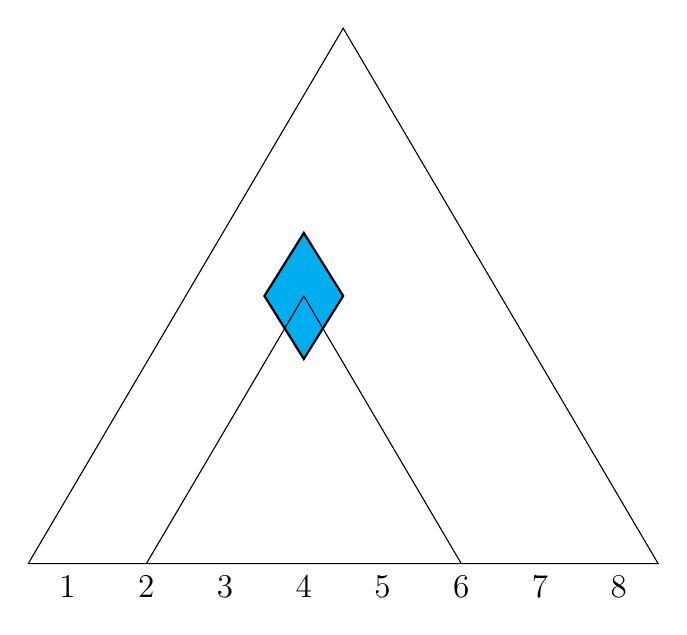
\begin{tikzpicture}
    \draw (0,0)--(8,0)--(4,6.8)--cycle;
    \fill[cyan] (3,3.4)--(3.5,2.6)--(4,3.4)--(3.5,4.2)--cycle;
    \draw[thick] (3,3.4)--(3.5,2.6)--(4,3.4)--(3.5,4.2)--cycle;
    
    \draw (3.5,3.4)--(1.5,0);
    \draw (3.5,3.4)--(5.5,0);


    \node[font=\large] at (0.5,-0.3) {$1$};
    \node[font=\large] at (1.5,-0.3) {$2$};
    \node[font=\large] at (2.5,-0.3) {$3$};
    \node[font=\large] at (3.5,-0.3) {$4$};
    \node[font=\large] at (4.5,-0.3) {$5$};
    \node[font=\large] at (5.5,-0.3) {$6$};
    \node[font=\large] at (6.5,-0.3) {$7$};
    \node[font=\large] at (7.5,-0.3) {$8$};
  \end{tikzpicture}

  $\text{wt}(p)=y_6-y_2$
\end{center}

\begin{defin}
  puzzle $P$に対してそのウェイト$\text{wt}(P)$を
  \[
  \text{wt}(P):=\prod_{p:\text{ equivariant piece}}\text{wt}(p)
  \]
  とする.
\end{defin}

式(\ref{LRcoeff})の係数$C^\nu_{\lambda\mu}$に関して次が成り立つ.

\begin{theo}(Knutson-Tao \cite{knutson tao})
  \[
  C^\nu_{\lambda\mu}=\prod_{\substack{P:\text{ puzzle} \\ \partial P = \Delta^\nu_{\lambda\mu}}}\text{wt}(P)
  \]
  が成り立つ.
\end{theo}



\subsection{edge labeled tableauxによる方法}

\begin{defin}
  $n$の分割$\lambda=(\lambda_1\geq\cdots\geq\lambda_k>0)$に対して,$1$行目に$\lambda_1$個の箱を, $2$行目に$\lambda_2$個の箱を,順に$k$行目まで左寄せで書いた図をYoung図形という.以降分割とYoung図形を同一視して同じ記号で表す.$\lambda$の各箱に,各行について左から右に単調増大, 各列について上から下に単調増大となるように相異なる数字を$1$回ずつ書き入れたものをstandard tableauxという.
\end{defin}

\begin{eg}
$\lambda=(5,3,3,1)$のYoung図形とその上のstandard tableauxの例
\[
\ytableausetup{nobaseline}
\ydiagram{5, 3, 3, 1}
\quad\begin{ytableau}
    1&3&5&6&12\\
    2&4&8\\
    7&9&10\\
    11
\end{ytableau}
\]
\end{eg}


\begin{defin}
  分割$\lambda, \mu$に対して,$\lambda\leq\mu\Leftrightarrow \lambda_i\leq\mu_i\:(\forall i)$によって順序を定める.$\lambda<\mu$を満たすYoung図形に対して,$\mu$のYoung図形から$\lambda$に相当する部分を取り除いた図形を歪Young図形といい$\mu/\lambda$で表す.整数$n>0$を固定する. 歪Young図形の各箱に$1$から$n$までの数字を書き入れ,水平方向の各辺に$\{1,\cdots,n\}$の部分集合(空でもよい)を書き入れたものを, equivariant fillingという.equivariant fillingのうち,次の条件を満たすものをequivariant standard tableauxという.
  \begin{itemize}
    \item $1$から$n$までの各数字が,いずれかの箱のラベルに現れるか,またはいずれかの辺のラベルの要素になっている.また$1$から$n$までの各数字がちょうど1回現れる.
    \item 各箱のラベルについて,左隣の箱のラベルよりも大きい.
    \item 各箱のラベルについて,上辺のラベルが空でないなら,その最大値よりも大きい.空であるならば,すぐ上の箱のラベルより大きい.
    \item 各辺のラベルについて,そのすべての数字がすぐ上の箱に書かれたラベルよりも大きい.
  \end{itemize}
  形が$\mu/\lambda$で$1$から$n$までの数字が書かれたequivariant standard tableauxの全体の集合を$\text{EqSYT}(\mu/\lambda, n)$とする.
\end{defin}

\begin{eg}\label{example of EqSYT}
  $(4,3,3,1)/(2,2,1)$上のequivariant standard tableauxの例(左図)と$(4,4,2)/(3,3,1)$上のequivariant standard tableauxの例(右図)
  \begin{center}
    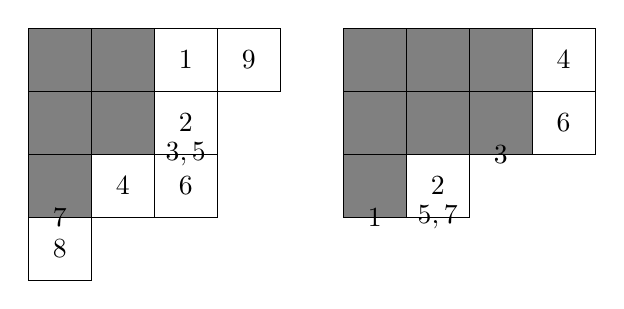
\begin{tikzpicture}
      \begin{scope}
        \fill[gray] (0,0)--(1.6,0)--(1.6,-1.6)--(0.8,-1.6)--(0.8,-2.4)--(0,-2.4)--cycle;
        \draw (0,0)--(0,-3.2)--(0.8,-3.2)--(0.8,-2.4)--(2.4,-2.4)--(2.4,-0.8)--(3.2,-0.8)--(3.2,0)--cycle;
        \draw (0,-0.8)--(2.4,-0.8);
        \draw (0,-1.6)--(2.4,-1.6);
        \draw (0,-2.4)--(0.8,-2.4);
        \draw (0.8,0)--(0.8,-2.4);
        \draw (1.6,0)--(1.6,-2.4);
        \draw (2.4,0)--(2.4,-0.8);
  
        \node at (2,-0.4) {$1$};
        \node at (2.8,-0.4) {$9$};
        \node at (2,-1.2) {$2$};
        \node at (1.2,-2) {$4$};
        \node at (2,-2) {$6$};
        \node at (0.4,-2.8) {$8$};
  
        \node at (0.4,-2.4) {$7$};
        \node at (2,-1.6) {$3,5$};
      \end{scope}
      \begin{scope}[xshift=4cm]
        \fill[gray] (0,0)--(2.4,0)--(2.4,-1.6)--(0.8,-1.6)--(0.8,-2.4)--(0,-2.4)--cycle;
        \draw (0,0)--(3.2,0)--(3.2,-1.6)--(1.6,-1.6)--(1.6,-2.4)--(0,-2.4)--cycle;
        \draw (0.8,0)-- +(0,-2.4);
        \draw (1.6,0)-- +(0,-1.6);
        \draw (2.4,0)-- +(0,-1.6);
        \draw (0,-0.8)-- +(3.2,0);
        \draw (0,-1.6)-- +(1.6,0);
  
        \node at (2.8,-0.4) {$4$};
        \node at (2.8,-1.2) {$6$};
        \node at (1.2,-2) {$2$};
        \node at (0.4,-2.4) {$1$};
        \node at (1.2,-2.4) {$5,7$};
        \node at (2,-1.6) {$3$};
      \end{scope}
    \end{tikzpicture}
  \end{center}
\end{eg}

\begin{defin}
  $\lambda$の箱$x$が$T\in\text{EqSYT}(\mu/\lambda, n)$の内隅であるとは,$x$のすぐ右とすぐ下の箱が$\lambda$の箱でないことをいう.また$\mu/\lambda$の箱$x$が外隅であるとは,$x$のすぐ右とすぐ下の箱が存在しないことをいう.$T$の内隅$x$に対して,次の操作を考える:
  \begin{enumerate}
    \item $x$の下辺のラベル$l$が空でないなら,$l$の最小値を$x$のラベルに移す
    \item $x$の下辺のラベルが空であるとし,$x$のすぐ右の箱を$y$,すぐ下の箱を$z$とする.$y$と$z$のうち,ラベルの小さい方の箱を$x$と交換する(このとき辺のラベルは交換しない).
  \end{enumerate}
  (i)の操作が行われる,もしくは$x$が外隅になるまで(i),(ii)を繰り返してできるtableauxを$T$の$x$によるequivariant jeu de taquin といい,$\text{EqJdt}_x(T)$と書く.
\end{defin}

\begin{defin}
  $\lambda$の箱を各列に沿って下から上に,右から左に数えて$x_1,\cdots,x_m$とする.$T\in\text{EqSYT}(\mu/\lambda, n)$に対して,$T$のequivariant rectificationを$x_1$から順に$x_m$までequivariant jeu de taquinを行って得られるtableauxとする.すなわち
  \[
  \text{EqRect}(T):=\text{EqJdt}_{x_m}(\text{EqJdt}_{x_{m-1}}(\cdots(\text{EqJdt}_{x_1}(T))\cdots))
  \]
  をTのequivariant rectificationという.
\end{defin}

\begin{eg}\label{fst calculation}
  例\ref{example of EqSYT}左図のtableauxのequivariant rectificationを図示する.
  \begin{center}
    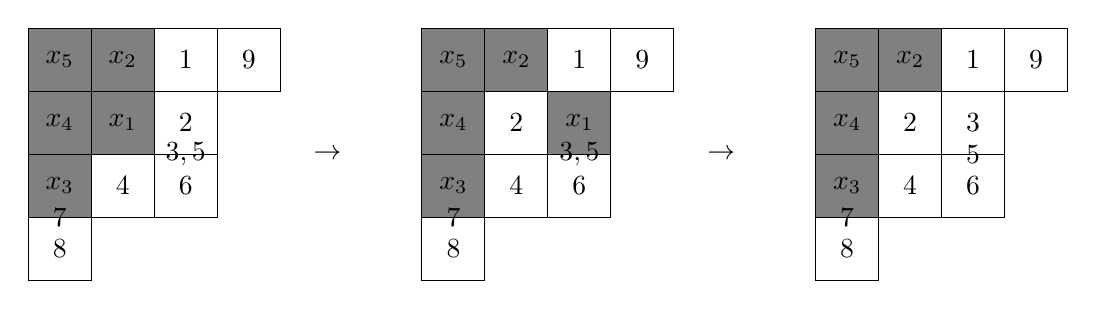
\begin{tikzpicture}
      \begin{scope}
        \fill[gray] (0,0)--(1.6,0)--(1.6,-1.6)--(0.8,-1.6)--(0.8,-2.4)--(0,-2.4)--cycle;
        \draw (0,0)--(0,-3.2)--(0.8,-3.2)--(0.8,-2.4)--(2.4,-2.4)--(2.4,-0.8)--(3.2,-0.8)--(3.2,0)--cycle;
        \draw (0,-0.8)--(2.4,-0.8);
        \draw (0,-1.6)--(2.4,-1.6);
        \draw (0,-2.4)--(0.8,-2.4);
        \draw (0.8,0)--(0.8,-2.4);
        \draw (1.6,0)--(1.6,-2.4);
        \draw (2.4,0)--(2.4,-0.8);
  
        \node at (2,-0.4) {$1$};
        \node at (2.8,-0.4) {$9$};
        \node at (2,-1.2) {$2$};
        \node at (1.2,-2) {$4$};
        \node at (2,-2) {$6$};
        \node at (0.4,-2.8) {$8$};
  
        \node at (0.4,-2.4) {$7$};
        \node at (2,-1.6) {$3,5$};

        \node at (1.2,-1.2) {$x_1$};
        \node at (1.2,-0.4) {$x_2$};
        \node at (0.4,-2) {$x_3$};
        \node at (0.4,-1.2) {$x_4$};
        \node at (0.4,-0.4) {$x_5$};
        \node at (3.8,-1.6) {$\rightarrow$};
      \end{scope}
      \begin{scope}[xshift=5cm]
        \fill[gray] (0,0)--(1.6,0)--(1.6,-0.8)--(0.8,-0.8)--(0.8,-2.4)--(0,-2.4)--cycle;
        \fill[gray] (1.6,-0.8) rectangle (2.4,-1.6);
        \draw (0,0)--(0,-3.2)--(0.8,-3.2)--(0.8,-2.4)--(2.4,-2.4)--(2.4,-0.8)--(3.2,-0.8)--(3.2,0)--cycle;
        \draw (0,-0.8)--(2.4,-0.8);
        \draw (0,-1.6)--(2.4,-1.6);
        \draw (0,-2.4)--(0.8,-2.4);
        \draw (0.8,0)--(0.8,-2.4);
        \draw (1.6,0)--(1.6,-2.4);
        \draw (2.4,0)--(2.4,-0.8);
  
        \node at (2,-0.4) {$1$};
        \node at (2.8,-0.4) {$9$};
        \node at (2,-1.2) {$x_1$};
        \node at (1.2,-2) {$4$};
        \node at (2,-2) {$6$};
        \node at (0.4,-2.8) {$8$};
  
        \node at (0.4,-2.4) {$7$};
        \node at (2,-1.6) {$3,5$};
        \node at (1.2,-1.2) {$2$};

        \node at (1.2,-0.4) {$x_2$};
        \node at (0.4,-2) {$x_3$};
        \node at (0.4,-1.2) {$x_4$};
        \node at (0.4,-0.4) {$x_5$};

        \node at (3.8,-1.6) {$\rightarrow$};
      \end{scope}
      \begin{scope}[xshift=10cm]
        \fill[gray] (0,0)--(1.6,0)--(1.6,-0.8)--(0.8,-0.8)--(0.8,-2.4)--(0,-2.4)--cycle;
        \draw (0,0)--(0,-3.2)--(0.8,-3.2)--(0.8,-2.4)--(2.4,-2.4)--(2.4,-0.8)--(3.2,-0.8)--(3.2,0)--cycle;
        \draw (0,-0.8)--(2.4,-0.8);
        \draw (0,-1.6)--(2.4,-1.6);
        \draw (0,-2.4)--(0.8,-2.4);
        \draw (0.8,0)--(0.8,-2.4);
        \draw (1.6,0)--(1.6,-2.4);
        \draw (2.4,0)--(2.4,-0.8);
  
        \node at (2,-0.4) {$1$};
        \node at (2.8,-0.4) {$9$};
        \node at (2,-1.2) {$3$};
        \node at (1.2,-2) {$4$};
        \node at (2,-2) {$6$};
        \node at (0.4,-2.8) {$8$};
  
        \node at (0.4,-2.4) {$7$};
        \node at (2,-1.6) {$5$};
        \node at (1.2,-1.2) {$2$};
        
        \node at (1.2,-0.4) {$x_2$};
        \node at (0.4,-2) {$x_3$};
        \node at (0.4,-1.2) {$x_4$};
        \node at (0.4,-0.4) {$x_5$};
      \end{scope}
    \end{tikzpicture}

    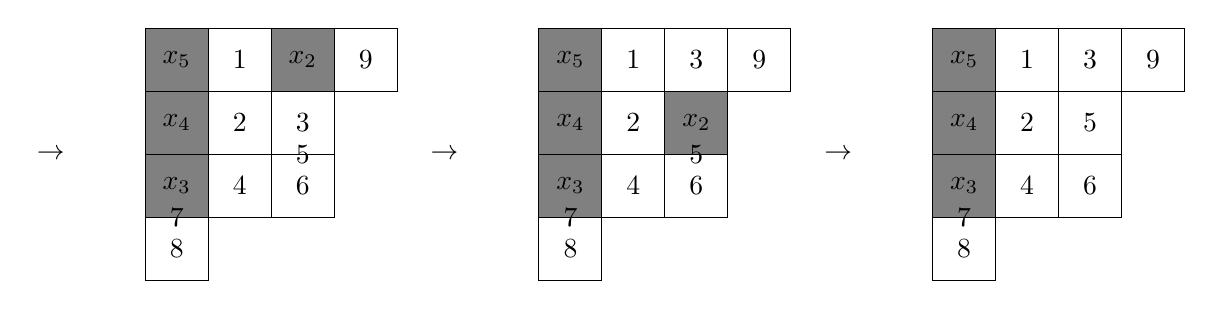
\begin{tikzpicture}
      \begin{scope}
        \fill[gray] (0,0)--(0.8,0)--(0.8,-2.4)--(0,-2.4)--cycle;
        \fill[gray] (1.6,0) rectangle (2.4,-0.8);
        \draw (0,0)--(0,-3.2)--(0.8,-3.2)--(0.8,-2.4)--(2.4,-2.4)--(2.4,-0.8)--(3.2,-0.8)--(3.2,0)--cycle;
        \draw (0,-0.8)--(2.4,-0.8);
        \draw (0,-1.6)--(2.4,-1.6);
        \draw (0,-2.4)--(0.8,-2.4);
        \draw (0.8,0)--(0.8,-2.4);
        \draw (1.6,0)--(1.6,-2.4);
        \draw (2.4,0)--(2.4,-0.8);
  
        \node at (2,-0.4) {$x_2$};
        \node at (2.8,-0.4) {$9$};
        \node at (2,-1.2) {$3$};
        \node at (1.2,-2) {$4$};
        \node at (2,-2) {$6$};
        \node at (0.4,-2.8) {$8$};
  
        \node at (0.4,-2.4) {$7$};
        \node at (2,-1.6) {$5$};
        \node at (1.2,-1.2) {$2$};
        
        \node at (1.2,-0.4) {$1$};
        \node at (0.4,-2) {$x_3$};
        \node at (0.4,-1.2) {$x_4$};
        \node at (0.4,-0.4) {$x_5$};
        \node at (-1.2,-1.6) {$\rightarrow $};
        \node at (3.8,-1.6) {$\rightarrow $};
      \end{scope}
      \begin{scope}[xshift=5cm]
        \fill[gray] (0,0)--(0.8,0)--(0.8,-2.4)--(0,-2.4)--cycle;
        \fill[gray] (1.6,-0.8) rectangle (2.4,-1.6);
        \draw (0,0)--(0,-3.2)--(0.8,-3.2)--(0.8,-2.4)--(2.4,-2.4)--(2.4,-0.8)--(3.2,-0.8)--(3.2,0)--cycle;
        \draw (0,-0.8)--(2.4,-0.8);
        \draw (0,-1.6)--(2.4,-1.6);
        \draw (0,-2.4)--(0.8,-2.4);
        \draw (0.8,0)--(0.8,-2.4);
        \draw (1.6,0)--(1.6,-2.4);
        \draw (2.4,0)--(2.4,-0.8);
  
        \node at (2,-0.4) {$3$};
        \node at (2.8,-0.4) {$9$};
        \node at (2,-1.2) {$x_2$};
        \node at (1.2,-2) {$4$};
        \node at (2,-2) {$6$};
        \node at (0.4,-2.8) {$8$};
  
        \node at (0.4,-2.4) {$7$};
        \node at (2,-1.6) {$5$};
        \node at (1.2,-1.2) {$2$};
        
        \node at (1.2,-0.4) {$1$};
        \node at (0.4,-2) {$x_3$};
        \node at (0.4,-1.2) {$x_4$};
        \node at (0.4,-0.4) {$x_5$};
        \node at (3.8,-1.6) {$\rightarrow $};
      \end{scope}
      \begin{scope}[xshift=10cm]
        \fill[gray] (0,0)--(0.8,0)--(0.8,-2.4)--(0,-2.4)--cycle;
        \draw (0,0)--(0,-3.2)--(0.8,-3.2)--(0.8,-2.4)--(2.4,-2.4)--(2.4,-0.8)--(3.2,-0.8)--(3.2,0)--cycle;
        \draw (0,-0.8)--(2.4,-0.8);
        \draw (0,-1.6)--(2.4,-1.6);
        \draw (0,-2.4)--(0.8,-2.4);
        \draw (0.8,0)--(0.8,-2.4);
        \draw (1.6,0)--(1.6,-2.4);
        \draw (2.4,0)--(2.4,-0.8);
  
        \node at (2,-0.4) {$3$};
        \node at (2.8,-0.4) {$9$};
        \node at (2,-1.2) {$5$};
        \node at (1.2,-2) {$4$};
        \node at (2,-2) {$6$};
        \node at (0.4,-2.8) {$8$};
  
        \node at (0.4,-2.4) {$7$};
        \node at (1.2,-1.2) {$2$};
        
        \node at (1.2,-0.4) {$1$};
        \node at (0.4,-2) {$x_3$};
        \node at (0.4,-1.2) {$x_4$};
        \node at (0.4,-0.4) {$x_5$};
      \end{scope}
    \end{tikzpicture}

    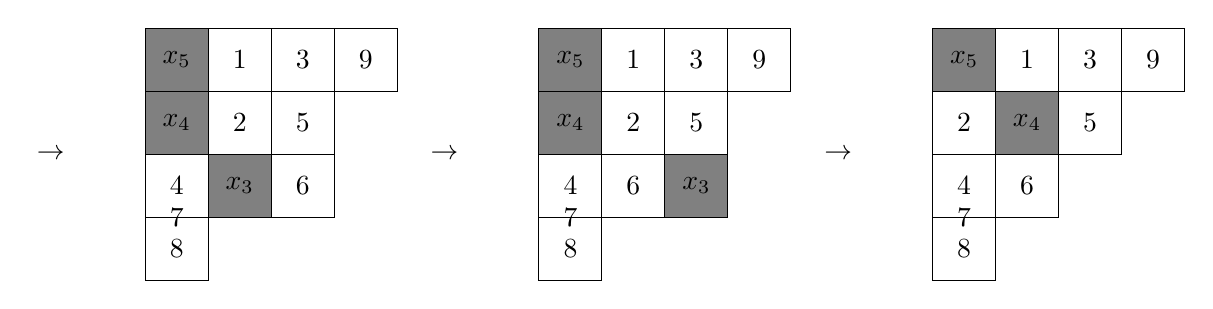
\begin{tikzpicture}
      \begin{scope}
        \fill[gray] (0,0) rectangle (0.8,-1.6);
        \fill[gray] (0.8,-1.6) rectangle (1.6,-2.4);
        \draw (0,0)--(0,-3.2)--(0.8,-3.2)--(0.8,-2.4)--(2.4,-2.4)--(2.4,-0.8)--(3.2,-0.8)--(3.2,0)--cycle;
        \draw (0,-0.8)--(2.4,-0.8);
        \draw (0,-1.6)--(2.4,-1.6);
        \draw (0,-2.4)--(0.8,-2.4);
        \draw (0.8,0)--(0.8,-2.4);
        \draw (1.6,0)--(1.6,-2.4);
        \draw (2.4,0)--(2.4,-0.8);
  
        \node at (2,-0.4) {$3$};
        \node at (2.8,-0.4) {$9$};
        \node at (2,-1.2) {$5$};
        \node at (1.2,-2) {$x_3$};
        \node at (2,-2) {$6$};
        \node at (0.4,-2.8) {$8$};
  
        \node at (1.2,-1.2) {$2$};
        
        \node at (1.2,-0.4) {$1$};
        \node at (0.4,-2) {$4$};
        \node at (0.4,-2.4) {$7$};
        \node at (0.4,-1.2) {$x_4$};
        \node at (0.4,-0.4) {$x_5$};
        \node at (-1.2,-1.6) {$\rightarrow $};
        \node at (3.8,-1.6) {$\rightarrow $};
      \end{scope}
      \begin{scope}[xshift=5cm]
        \fill[gray] (0,0) rectangle (0.8,-1.6);
        \fill[gray] (1.6,-1.6) rectangle (2.4,-2.4);
        \draw (0,0)--(0,-3.2)--(0.8,-3.2)--(0.8,-2.4)--(2.4,-2.4)--(2.4,-0.8)--(3.2,-0.8)--(3.2,0)--cycle;
        \draw (0,-0.8)--(2.4,-0.8);
        \draw (0,-1.6)--(2.4,-1.6);
        \draw (0,-2.4)--(0.8,-2.4);
        \draw (0.8,0)--(0.8,-2.4);
        \draw (1.6,0)--(1.6,-2.4);
        \draw (2.4,0)--(2.4,-0.8);
  
        \node at (2,-0.4) {$3$};
        \node at (2.8,-0.4) {$9$};
        \node at (2,-1.2) {$5$};
        \node at (1.2,-2) {$6$};
        \node at (2,-2) {$x_3$};
        \node at (0.4,-2.8) {$8$};
  
        \node at (1.2,-1.2) {$2$};
        
        \node at (1.2,-0.4) {$1$};
        \node at (0.4,-2) {$4$};
        \node at (0.4,-2.4) {$7$};
        \node at (0.4,-1.2) {$x_4$};
        \node at (0.4,-0.4) {$x_5$};
        \node at (3.8,-1.6) {$\rightarrow $};
      \end{scope}
      \begin{scope}[xshift=10cm]
        \fill[gray] (0,0) rectangle (0.8,-0.8);
        \fill[gray] (0.8,-0.8) rectangle (1.6,-1.6);
        \draw (0,0)--(0,-3.2)--(0.8,-3.2)--(0.8,-2.4)--(1.6,-2.4)--(1.6,-1.6)--(2.4,-1.6)--(2.4,-0.8)--(3.2,-0.8)--(3.2,0)--cycle;
        \draw (0,-0.8)--(2.4,-0.8);
        \draw (0,-1.6)--(2.4,-1.6);
        \draw (0,-2.4)--(0.8,-2.4);
        \draw (0.8,0)--(0.8,-2.4);
        \draw (1.6,0)--(1.6,-2.4);
        \draw (2.4,0)--(2.4,-0.8);
  
        \node at (2,-0.4) {$3$};
        \node at (2.8,-0.4) {$9$};
        \node at (2,-1.2) {$5$};
        \node at (1.2,-2) {$6$};
        \node at (0.4,-2.8) {$8$};
  
        \node at (1.2,-1.2) {$x_4$};
        
        \node at (1.2,-0.4) {$1$};
        \node at (0.4,-2) {$4$};
        \node at (0.4,-2.4) {$7$};
        \node at (0.4,-1.2) {$2$};
        \node at (0.4,-0.4) {$x_5$};
      \end{scope}
    \end{tikzpicture}

    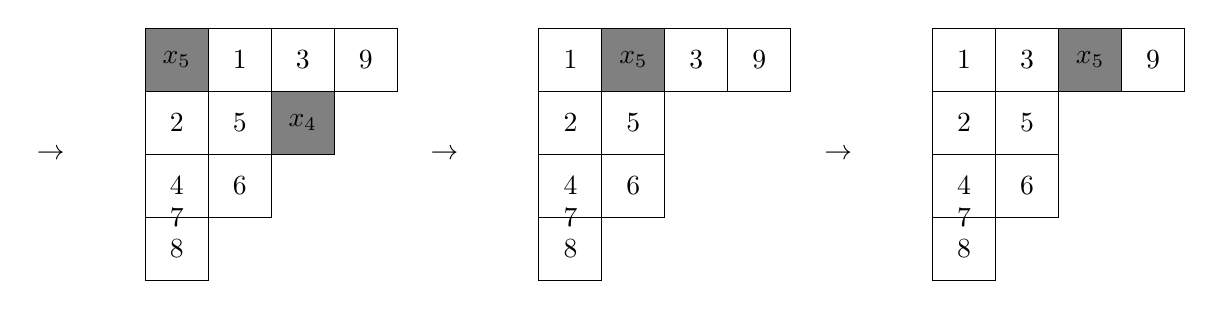
\begin{tikzpicture}
      \begin{scope}
        \fill[gray] (0,0) rectangle (0.8,-0.8);
        \fill[gray] (1.6,-0.8) rectangle (2.4,-1.6);
        \draw (0,0)--(0,-3.2)--(0.8,-3.2)--(0.8,-2.4)--(1.6,-2.4)--(1.6,-1.6)--(2.4,-1.6)--(2.4,-0.8)--(3.2,-0.8)--(3.2,0)--cycle;
        \draw (0,-0.8)--(2.4,-0.8);
        \draw (0,-1.6)--(2.4,-1.6);
        \draw (0,-2.4)--(0.8,-2.4);
        \draw (0.8,0)--(0.8,-2.4);
        \draw (1.6,0)--(1.6,-2.4);
        \draw (2.4,0)--(2.4,-0.8);
  
        \node at (2,-0.4) {$3$};
        \node at (2.8,-0.4) {$9$};
        \node at (2,-1.2) {$x_4$};
        \node at (1.2,-2) {$6$};
        \node at (0.4,-2.8) {$8$};
  
        \node at (1.2,-1.2) {$5$};
        
        \node at (1.2,-0.4) {$1$};
        \node at (0.4,-2) {$4$};
        \node at (0.4,-2.4) {$7$};
        \node at (0.4,-1.2) {$2$};
        \node at (0.4,-0.4) {$x_5$};

        \node at (-1.2,-1.6) {$\rightarrow $};
        \node at (3.8,-1.6) {$\rightarrow $};
      \end{scope}
      \begin{scope}[xshift=5cm]
        \fill[gray] (0.8,0) rectangle (1.6,-0.8);
        \draw (0,0)--(0,-3.2)--(0.8,-3.2)--(0.8,-2.4)--(1.6,-2.4)--(1.6,-0.8)--(3.2,-0.8)--(3.2,0)--cycle;
        \draw (0,-0.8)--(2.4,-0.8);
        \draw (0,-1.6)--(1.6,-1.6);
        \draw (0,-2.4)--(0.8,-2.4);
        \draw (0.8,0)--(0.8,-2.4);
        \draw (1.6,0)--(1.6,-2.4);
        \draw (2.4,0)--(2.4,-0.8);
  
        \node at (2,-0.4) {$3$};
        \node at (2.8,-0.4) {$9$};
        \node at (1.2,-2) {$6$};
        \node at (0.4,-2.8) {$8$};
  
        \node at (1.2,-1.2) {$5$};
        
        \node at (1.2,-0.4) {$x_5$};
        \node at (0.4,-2) {$4$};
        \node at (0.4,-2.4) {$7$};
        \node at (0.4,-1.2) {$2$};
        \node at (0.4,-0.4) {$1$};

        \node at (3.8,-1.6) {$\rightarrow $};
      \end{scope}
      \begin{scope}[xshift=10cm]
        \fill[gray] (1.6,0) rectangle (2.4,-0.8);
        \draw (0,0)--(0,-3.2)--(0.8,-3.2)--(0.8,-2.4)--(1.6,-2.4)--(1.6,-0.8)--(3.2,-0.8)--(3.2,0)--cycle;
        \draw (0,-0.8)--(2.4,-0.8);
        \draw (0,-1.6)--(1.6,-1.6);
        \draw (0,-2.4)--(0.8,-2.4);
        \draw (0.8,0)--(0.8,-2.4);
        \draw (1.6,0)--(1.6,-2.4);
        \draw (2.4,0)--(2.4,-0.8);
  
        \node at (2,-0.4) {$x_5$};
        \node at (2.8,-0.4) {$9$};
        \node at (1.2,-2) {$6$};
        \node at (0.4,-2.8) {$8$};
  
        \node at (1.2,-1.2) {$5$};
        
        \node at (1.2,-0.4) {$3$};
        \node at (0.4,-2) {$4$};
        \node at (0.4,-2.4) {$7$};
        \node at (0.4,-1.2) {$2$};
        \node at (0.4,-0.4) {$1$};
      \end{scope}
    \end{tikzpicture}

    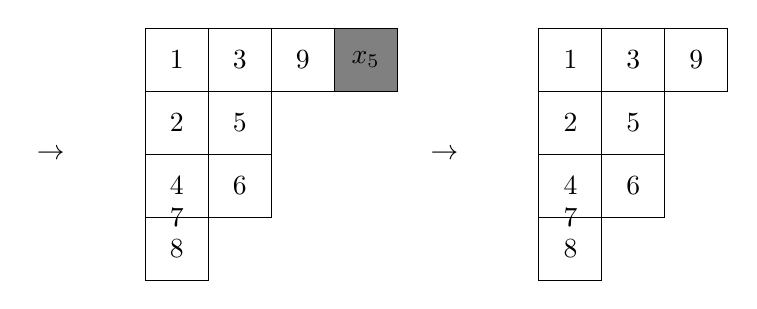
\begin{tikzpicture}
      \begin{scope}
        \fill[gray] (2.4,0) rectangle (3.2,-0.8);
        \draw (0,0)--(0,-3.2)--(0.8,-3.2)--(0.8,-2.4)--(1.6,-2.4)--(1.6,-0.8)--(3.2,-0.8)--(3.2,0)--cycle;
        \draw (0,-0.8)--(2.4,-0.8);
        \draw (0,-1.6)--(1.6,-1.6);
        \draw (0,-2.4)--(0.8,-2.4);
        \draw (0.8,0)--(0.8,-2.4);
        \draw (1.6,0)--(1.6,-2.4);
        \draw (2.4,0)--(2.4,-0.8);
  
        \node at (2,-0.4) {$9$};
        \node at (2.8,-0.4) {$x_5$};
        \node at (1.2,-2) {$6$};
        \node at (0.4,-2.8) {$8$};
  
        \node at (1.2,-1.2) {$5$};
        
        \node at (1.2,-0.4) {$3$};
        \node at (0.4,-2) {$4$};
        \node at (0.4,-2.4) {$7$};
        \node at (0.4,-1.2) {$2$};
        \node at (0.4,-0.4) {$1$};
        
        \node at (-1.2,-1.6) {$\rightarrow $};
        \node at (3.8,-1.6) {$\rightarrow $};
      \end{scope}
      \begin{scope}[xshift=5cm]
        \draw (0,0)--(0,-3.2)--(0.8,-3.2)--(0.8,-2.4)--(1.6,-2.4)--(1.6,-0.8)--(2.4,-0.8)--(2.4,0)--cycle;
        \draw (0,-0.8)--(2.4,-0.8);
        \draw (0,-1.6)--(1.6,-1.6);
        \draw (0,-2.4)--(0.8,-2.4);
        \draw (0.8,0)--(0.8,-2.4);
        \draw (1.6,0)--(1.6,-2.4);
        \draw (2.4,0)--(2.4,-0.8);
  
        \node at (2,-0.4) {$9$};
        \node at (1.2,-2) {$6$};
        \node at (0.4,-2.8) {$8$};
  
        \node at (1.2,-1.2) {$5$};
        
        \node at (1.2,-0.4) {$3$};
        \node at (0.4,-2) {$4$};
        \node at (0.4,-2.4) {$7$};
        \node at (0.4,-1.2) {$2$};
        \node at (0.4,-0.4) {$1$};
      \end{scope}
    \end{tikzpicture}
  \end{center}
\end{eg}

次に$T\in\text{EdSYT}(\mu/\lambda, n)$に対してそのウェイトを定義する.

\begin{defin}
  正の整数$m, k$を固定する.$\Lambda=\overbrace{(m,\cdots,m)}^{k\text{-copies}}$とする.$\Lambda$の箱$x$に対して
  \[
  \beta(x)=y_{i+1}-y_i\in \integer[y_1,\cdots,y_{m+k}]
  \]
  とする.ここで$i$は$\Lambda$の右上の隅の箱から$x$までのManhattan距離である.図は$k=3,m=4$における$\Lambda$の各箱のManhattan距離である.
  \[
  \begin{ytableau}
    4 & 3 & 2 & 1\\
    5 & 4 & 3 & 2\\
    6 & 5 & 4 & 3
  \end{ytableau}
  \]
\end{defin}

\begin{defin}
  $T\in\text{EqSYT}(\mu/\lambda, n), (\mu\leq\Lambda=\overbrace{(m,\cdots,m)}^{k\text{-copies}})$を固定し,$l$を$T$の辺のラベルに含まれる要素とする.$\text{factor}(l)\in\integer[y_1,\cdots,y_{m+k}]$を次のように定義する.$\text{EqRect}(T)$を計算する過程において,
  \begin{enumerate}
    \item $l$が含まれる列にある$\lambda$の箱をすべてequivariant jeu de taquinしたあとも,$l$が辺のラベルであるなら$\text{factor}(l)=0$とする.また$l$が含まれる列に$\lambda$の箱がない場合も$\text{factor}(l)=0$とする.
    \item $l$が含まれる列にある$\lambda$の箱をすべてequivariant jeu de taquinするとき,$l$が通った箱を下から順に$x_1,\cdots,x_s$とする.$x_s$と同じ行で$x_s$の右側にある$T$の箱を左から順に$y_1,\cdots,y_t$とする.このとき$\text{factor}(l)=\beta(x_1)+\cdots+\beta(x_s)+\beta(y_1)+\cdots+\beta(y_t)$とする.
  \end{enumerate}
\end{defin}

\begin{defin}
  $T\in\text{EqSYT}(\mu/\lambda, n)$に対して
  \[
  \text{wt}(T)=\prod_{l:\text{ edge label}}\text{factor}(l)
  \]
  とする.
\end{defin}

\begin{eg}
  例\ref{fst calculation}の計算より,
  \begin{center}
    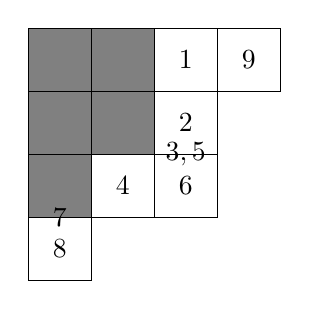
\begin{tikzpicture}
      \fill[gray] (0,0)--(1.6,0)--(1.6,-1.6)--(0.8,-1.6)--(0.8,-2.4)--(0,-2.4)--cycle;
        \draw (0,0)--(0,-3.2)--(0.8,-3.2)--(0.8,-2.4)--(2.4,-2.4)--(2.4,-0.8)--(3.2,-0.8)--(3.2,0)--cycle;
        \draw (0,-0.8)--(2.4,-0.8);
        \draw (0,-1.6)--(2.4,-1.6);
        \draw (0,-2.4)--(0.8,-2.4);
        \draw (0.8,0)--(0.8,-2.4);
        \draw (1.6,0)--(1.6,-2.4);
        \draw (2.4,0)--(2.4,-0.8);
  
        \node at (2,-0.4) {$1$};
        \node at (2.8,-0.4) {$9$};
        \node at (2,-1.2) {$2$};
        \node at (1.2,-2) {$4$};
        \node at (2,-2) {$6$};
        \node at (0.4,-2.8) {$8$};
  
        \node at (0.4,-2.4) {$7$};
        \node at (2,-1.6) {$3,5$};
    \end{tikzpicture}
  \end{center}
  のウェイトは
  \[
  \text{factor}(3)=\text{factor}(5)=\text{factor}(7)=0
  \]
  より$0$である.
\end{eg}

\begin{eg}
  例\ref{example of EqSYT}右図のtableauxのequivariant rectificationを図示する.
  \begin{center}
    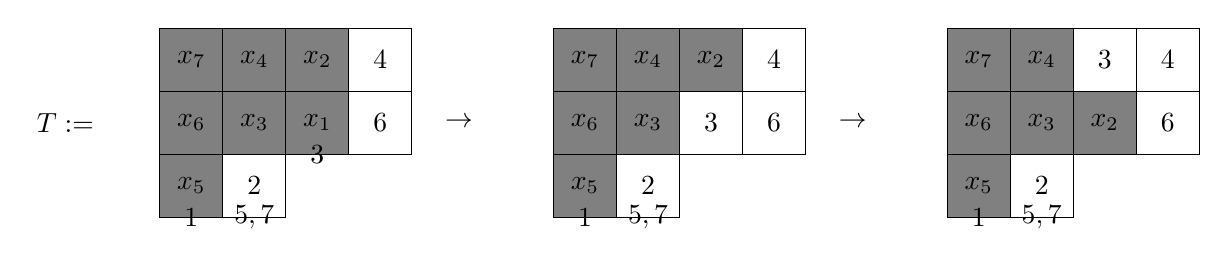
\begin{tikzpicture}
      \begin{scope}
        \fill[gray] (0,0)--(2.4,0)--(2.4,-1.6)--(0.8,-1.6)--(0.8,-2.4)--(0,-2.4)--cycle;
        \draw (0,0)--(3.2,0)--(3.2,-1.6)--(1.6,-1.6)--(1.6,-2.4)--(0,-2.4)--cycle;
        \draw (0.8,0)-- +(0,-2.4);
        \draw (1.6,0)-- +(0,-1.6);
        \draw (2.4,0)-- +(0,-1.6);
        \draw (0,-0.8)-- +(3.2,0);
        \draw (0,-1.6)-- +(1.6,0);
  
        \node at (2.8,-0.4) {$4$};
        \node at (2.8,-1.2) {$6$};
        \node at (1.2,-2) {$2$};
        \node at (0.4,-2.4) {$1$};
        \node at (1.2,-2.4) {$5,7$};
        \node at (2,-1.6) {$3$};

        \node at (2,-1.2) {$x_1$};
        \node at (2,-0.4) {$x_2$};
        \node at (1.2,-1.2) {$x_3$};
        \node at (1.2,-0.4) {$x_4$};
        \node at (0.4,-2) {$x_5$};
        \node at (0.4,-1.2) {$x_6$};
        \node at (0.4,-0.4) {$x_7$};

        \node at (-1.2,-1.2) {$T:=$};
        \node at (3.8,-1.2) {$\rightarrow $};
      \end{scope}
      \begin{scope}[xshift=5cm]
        \fill[gray] (0,0)--(2.4,0)--(2.4,-0.8)--(1.6,-0.8)--(1.6,-1.6)--(0.8,-1.6)--(0.8,-2.4)--(0,-2.4)--cycle;
        \draw (0,0)--(3.2,0)--(3.2,-1.6)--(1.6,-1.6)--(1.6,-2.4)--(0,-2.4)--cycle;
        \draw (0.8,0)-- +(0,-2.4);
        \draw (1.6,0)-- +(0,-1.6);
        \draw (2.4,0)-- +(0,-1.6);
        \draw (0,-0.8)-- +(3.2,0);
        \draw (0,-1.6)-- +(1.6,0);
  
        \node at (2.8,-0.4) {$4$};
        \node at (2.8,-1.2) {$6$};
        \node at (1.2,-2) {$2$};
        \node at (0.4,-2.4) {$1$};
        \node at (1.2,-2.4) {$5,7$};

        \node at (2,-1.2) {$3$};
        \node at (2,-0.4) {$x_2$};
        \node at (1.2,-1.2) {$x_3$};
        \node at (1.2,-0.4) {$x_4$};
        \node at (0.4,-2) {$x_5$};
        \node at (0.4,-1.2) {$x_6$};
        \node at (0.4,-0.4) {$x_7$};

        \node at (3.8,-1.2) {$\rightarrow $};
      \end{scope}
      \begin{scope}[xshift=10cm]
        \fill[gray] (0,0)--(1.6,0)--(1.6,-1.6)--(0.8,-1.6)--(0.8,-2.4)--(0,-2.4)--cycle;
        \fill[gray] (1.6,-0.8) rectangle (2.4,-1.6);
        \draw (0,0)--(3.2,0)--(3.2,-1.6)--(1.6,-1.6)--(1.6,-2.4)--(0,-2.4)--cycle;
        \draw (0.8,0)-- +(0,-2.4);
        \draw (1.6,0)-- +(0,-1.6);
        \draw (2.4,0)-- +(0,-1.6);
        \draw (0,-0.8)-- +(3.2,0);
        \draw (0,-1.6)-- +(1.6,0);
  
        \node at (2.8,-0.4) {$4$};
        \node at (2.8,-1.2) {$6$};
        \node at (1.2,-2) {$2$};
        \node at (0.4,-2.4) {$1$};
        \node at (1.2,-2.4) {$5,7$};

        \node at (2,-1.2) {$x_2$};
        \node at (2,-0.4) {$3$};
        \node at (1.2,-1.2) {$x_3$};
        \node at (1.2,-0.4) {$x_4$};
        \node at (0.4,-2) {$x_5$};
        \node at (0.4,-1.2) {$x_6$};
        \node at (0.4,-0.4) {$x_7$};
      \end{scope}
    \end{tikzpicture}

    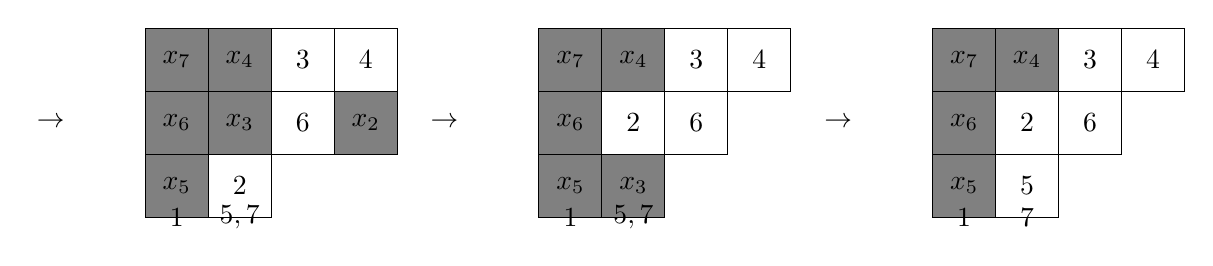
\begin{tikzpicture}
      \begin{scope}
        \fill[gray] (0,0)--(1.6,0)--(1.6,-1.6)--(0.8,-1.6)--(0.8,-2.4)--(0,-2.4)--cycle;
        \fill[gray] (2.4,-0.8) rectangle (3.2,-1.6);
        \draw (0,0)--(3.2,0)--(3.2,-1.6)--(1.6,-1.6)--(1.6,-2.4)--(0,-2.4)--cycle;
        \draw (0.8,0)-- +(0,-2.4);
        \draw (1.6,0)-- +(0,-1.6);
        \draw (2.4,0)-- +(0,-1.6);
        \draw (0,-0.8)-- +(3.2,0);
        \draw (0,-1.6)-- +(1.6,0);
  
        \node at (2.8,-0.4) {$4$};
        \node at (2.8,-1.2) {$x_2$};
        \node at (1.2,-2) {$2$};
        \node at (0.4,-2.4) {$1$};
        \node at (1.2,-2.4) {$5,7$};

        \node at (2,-1.2) {$6$};
        \node at (2,-0.4) {$3$};
        \node at (1.2,-1.2) {$x_3$};
        \node at (1.2,-0.4) {$x_4$};
        \node at (0.4,-2) {$x_5$};
        \node at (0.4,-1.2) {$x_6$};
        \node at (0.4,-0.4) {$x_7$};

        \node at (-1.2,-1.2) {$\rightarrow $};
        \node at (3.8,-1.2) {$\rightarrow $};
      \end{scope}
      \begin{scope}[xshift=5cm]
        \fill[gray] (0,0)--(1.6,0)--(1.6,-0.8)--(0.8,-0.8)--(0.8,-2.4)--(0,-2.4)--cycle;
        \fill[gray] (0.8,-1.6) rectangle (1.6,-2.4);
        \draw (0,0)--(3.2,0)--(3.2,-0.8)--(2.4,-0.8)--(2.4,-1.6)--(1.6,-1.6)--(1.6,-2.4)--(0,-2.4)--cycle;
        \draw (0.8,0)-- +(0,-2.4);
        \draw (1.6,0)-- +(0,-1.6);
        \draw (2.4,0)-- +(0,-1.6);
        \draw (0,-0.8)-- +(3.2,0);
        \draw (0,-1.6)-- +(1.6,0);
  
        \node at (2.8,-0.4) {$4$};
        \node at (1.2,-2) {$x_3$};
        \node at (0.4,-2.4) {$1$};
        \node at (1.2,-2.4) {$5,7$};

        \node at (2,-1.2) {$6$};
        \node at (2,-0.4) {$3$};
        \node at (1.2,-1.2) {$2$};
        \node at (1.2,-0.4) {$x_4$};
        \node at (0.4,-2) {$x_5$};
        \node at (0.4,-1.2) {$x_6$};
        \node at (0.4,-0.4) {$x_7$};

        \node at (3.8,-1.2) {$\rightarrow $};
      \end{scope}
      \begin{scope}[xshift=10cm]
        \fill[gray] (0,0)--(1.6,0)--(1.6,-0.8)--(0.8,-0.8)--(0.8,-2.4)--(0,-2.4)--cycle;
        \draw (0,0)--(3.2,0)--(3.2,-0.8)--(2.4,-0.8)--(2.4,-1.6)--(1.6,-1.6)--(1.6,-2.4)--(0,-2.4)--cycle;
        \draw (0.8,0)-- +(0,-2.4);
        \draw (1.6,0)-- +(0,-1.6);
        \draw (2.4,0)-- +(0,-1.6);
        \draw (0,-0.8)-- +(3.2,0);
        \draw (0,-1.6)-- +(1.6,0);
  
        \node at (2.8,-0.4) {$4$};
        \node at (1.2,-2) {$5$};
        \node at (0.4,-2.4) {$1$};
        \node at (1.2,-2.4) {$7$};

        \node at (2,-1.2) {$6$};
        \node at (2,-0.4) {$3$};
        \node at (1.2,-1.2) {$2$};
        \node at (1.2,-0.4) {$x_4$};
        \node at (0.4,-2) {$x_5$};
        \node at (0.4,-1.2) {$x_6$};
        \node at (0.4,-0.4) {$x_7$};
      \end{scope}
    \end{tikzpicture}

    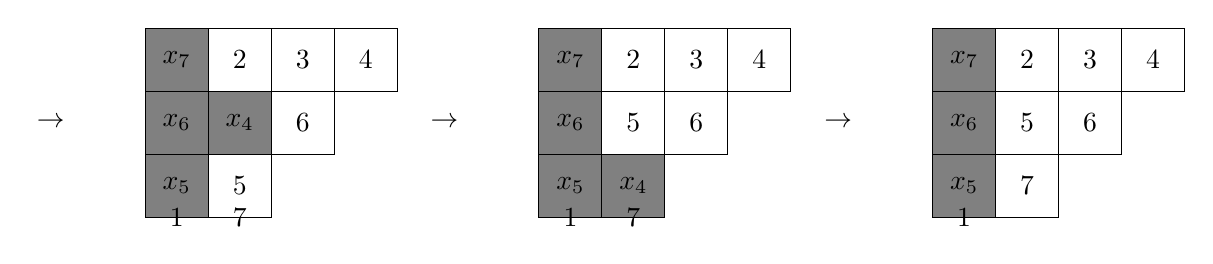
\begin{tikzpicture}
      \begin{scope}
        \fill[gray] (0,0)--(0.8,0)--(0.8,-2.4)--(0,-2.4)--cycle;
        \fill[gray] (0.8,-0.8) rectangle (1.6,-1.6);
        \draw (0,0)--(3.2,0)--(3.2,-0.8)--(2.4,-0.8)--(2.4,-1.6)--(1.6,-1.6)--(1.6,-2.4)--(0,-2.4)--cycle;
        \draw (0.8,0)-- +(0,-2.4);
        \draw (1.6,0)-- +(0,-1.6);
        \draw (2.4,0)-- +(0,-1.6);
        \draw (0,-0.8)-- +(3.2,0);
        \draw (0,-1.6)-- +(1.6,0);
  
        \node at (2.8,-0.4) {$4$};
        \node at (1.2,-2) {$5$};
        \node at (0.4,-2.4) {$1$};
        \node at (1.2,-2.4) {$7$};

        \node at (2,-1.2) {$6$};
        \node at (2,-0.4) {$3$};
        \node at (1.2,-1.2) {$x_4$};
        \node at (1.2,-0.4) {$2$};
        \node at (0.4,-2) {$x_5$};
        \node at (0.4,-1.2) {$x_6$};
        \node at (0.4,-0.4) {$x_7$};

        \node at (-1.2,-1.2) {$\rightarrow $};
        \node at (3.8,-1.2) {$\rightarrow $};
      \end{scope}
      \begin{scope}[xshift=5cm]
        \fill[gray] (0,0)--(0.8,0)--(0.8,-2.4)--(0,-2.4)--cycle;
        \fill[gray] (0.8,-1.6) rectangle (1.6,-2.4);
        \draw (0,0)--(3.2,0)--(3.2,-0.8)--(2.4,-0.8)--(2.4,-1.6)--(1.6,-1.6)--(1.6,-2.4)--(0,-2.4)--cycle;
        \draw (0.8,0)-- +(0,-2.4);
        \draw (1.6,0)-- +(0,-1.6);
        \draw (2.4,0)-- +(0,-1.6);
        \draw (0,-0.8)-- +(3.2,0);
        \draw (0,-1.6)-- +(1.6,0);
  
        \node at (2.8,-0.4) {$4$};
        \node at (1.2,-2) {$x_4$};
        \node at (0.4,-2.4) {$1$};
        \node at (1.2,-2.4) {$7$};

        \node at (2,-1.2) {$6$};
        \node at (2,-0.4) {$3$};
        \node at (1.2,-1.2) {$5$};
        \node at (1.2,-0.4) {$2$};
        \node at (0.4,-2) {$x_5$};
        \node at (0.4,-1.2) {$x_6$};
        \node at (0.4,-0.4) {$x_7$};

        \node at (3.8,-1.2) {$\rightarrow $};
      \end{scope}
      \begin{scope}[xshift=10cm]
        \fill[gray] (0,0)--(0.8,0)--(0.8,-2.4)--(0,-2.4)--cycle;
        \draw (0,0)--(3.2,0)--(3.2,-0.8)--(2.4,-0.8)--(2.4,-1.6)--(1.6,-1.6)--(1.6,-2.4)--(0,-2.4)--cycle;
        \draw (0.8,0)-- +(0,-2.4);
        \draw (1.6,0)-- +(0,-1.6);
        \draw (2.4,0)-- +(0,-1.6);
        \draw (0,-0.8)-- +(3.2,0);
        \draw (0,-1.6)-- +(1.6,0);
  
        \node at (2.8,-0.4) {$4$};
        \node at (1.2,-2) {$7$};
        \node at (0.4,-2.4) {$1$};

        \node at (2,-1.2) {$6$};
        \node at (2,-0.4) {$3$};
        \node at (1.2,-1.2) {$5$};
        \node at (1.2,-0.4) {$2$};
        \node at (0.4,-2) {$x_5$};
        \node at (0.4,-1.2) {$x_6$};
        \node at (0.4,-0.4) {$x_7$};
      \end{scope}
    \end{tikzpicture}

    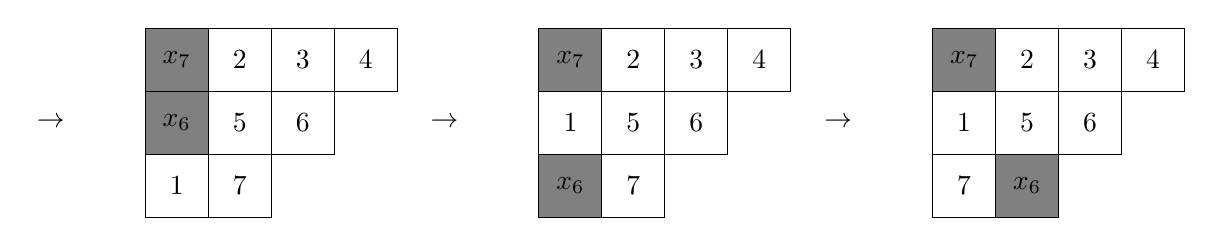
\begin{tikzpicture}
      \fill[gray] (0,0) rectangle (0.8,-1.6);
      \draw (0,0)--(3.2,0)--(3.2,-0.8)--(2.4,-0.8)--(2.4,-1.6)--(1.6,-1.6)--(1.6,-2.4)--(0,-2.4)--cycle;
      \draw (0.8,0)-- +(0,-2.4);
      \draw (1.6,0)-- +(0,-1.6);
      \draw (2.4,0)-- +(0,-1.6);
      \draw (0,-0.8)-- +(3.2,0);
      \draw (0,-1.6)-- +(1.6,0);

      \node at (2.8,-0.4) {$4$};
      \node at (1.2,-2) {$7$};
      \node at (2,-1.2) {$6$};
      \node at (2,-0.4) {$3$};
      \node at (1.2,-1.2) {$5$};
      \node at (1.2,-0.4) {$2$};
      \node at (0.4,-2) {$1$};
      \node at (0.4,-1.2) {$x_6$};
      \node at (0.4,-0.4) {$x_7$};

      \node at (-1.2,-1.2) {$\rightarrow $};
      \node at (3.8,-1.2) {$\rightarrow $};
      \begin{scope}[xshift=5cm]
        \fill[gray] (0,0) rectangle (0.8,-0.8);
        \fill[gray] (0,-1.6) rectangle (0.8,-2.4);
        \draw (0,0)--(3.2,0)--(3.2,-0.8)--(2.4,-0.8)--(2.4,-1.6)--(1.6,-1.6)--(1.6,-2.4)--(0,-2.4)--cycle;
        \draw (0.8,0)-- +(0,-2.4);
        \draw (1.6,0)-- +(0,-1.6);
        \draw (2.4,0)-- +(0,-1.6);
        \draw (0,-0.8)-- +(3.2,0);
        \draw (0,-1.6)-- +(1.6,0);

        \node at (2.8,-0.4) {$4$};
        \node at (1.2,-2) {$7$};
        \node at (2,-1.2) {$6$};
        \node at (2,-0.4) {$3$};
        \node at (1.2,-1.2) {$5$};
        \node at (1.2,-0.4) {$2$};
        \node at (0.4,-2) {$x_6$};
        \node at (0.4,-1.2) {$1$};
        \node at (0.4,-0.4) {$x_7$};

        \node at (3.8,-1.2) {$\rightarrow $};
      \end{scope}
      \begin{scope}[xshift=10cm]
        \fill[gray] (0,0) rectangle (0.8,-0.8);
        \fill[gray] (0.8,-1.6) rectangle (1.6,-2.4);
        \draw (0,0)--(3.2,0)--(3.2,-0.8)--(2.4,-0.8)--(2.4,-1.6)--(1.6,-1.6)--(1.6,-2.4)--(0,-2.4)--cycle;
        \draw (0.8,0)-- +(0,-2.4);
        \draw (1.6,0)-- +(0,-1.6);
        \draw (2.4,0)-- +(0,-1.6);
        \draw (0,-0.8)-- +(3.2,0);
        \draw (0,-1.6)-- +(1.6,0);

        \node at (2.8,-0.4) {$4$};
        \node at (1.2,-2) {$x_6$};
        \node at (2,-1.2) {$6$};
        \node at (2,-0.4) {$3$};
        \node at (1.2,-1.2) {$5$};
        \node at (1.2,-0.4) {$2$};
        \node at (0.4,-2) {$7$};
        \node at (0.4,-1.2) {$1$};
        \node at (0.4,-0.4) {$x_7$};
      \end{scope}
    \end{tikzpicture}

    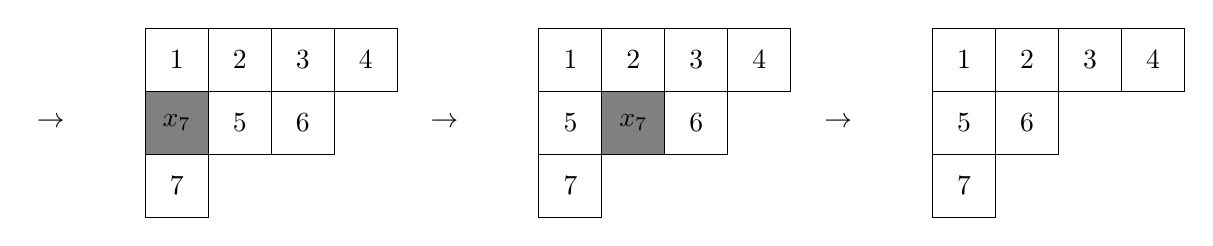
\begin{tikzpicture}
      \begin{scope}
        \fill[gray] (0,-0.8) rectangle (0.8,-1.6);
        \draw (0,0)--(3.2,0)--(3.2,-0.8)--(2.4,-0.8)--(2.4,-1.6)--(0.8,-1.6)--(0.8,-2.4)--(0,-2.4)--cycle;
        \draw (0.8,0)-- +(0,-2.4);
        \draw (1.6,0)-- +(0,-1.6);
        \draw (2.4,0)-- +(0,-1.6);
        \draw (0,-0.8)-- +(3.2,0);
        \draw (0,-1.6)-- +(1.6,0);

        \node at (2.8,-0.4) {$4$};
        \node at (2,-1.2) {$6$};
        \node at (2,-0.4) {$3$};
        \node at (1.2,-1.2) {$5$};
        \node at (1.2,-0.4) {$2$};
        \node at (0.4,-2) {$7$};
        \node at (0.4,-1.2) {$x_7$};
        \node at (0.4,-0.4) {$1$};

        \node at (-1.2,-1.2) {$\rightarrow $};
        \node at (3.8,-1.2) {$\rightarrow $};
      \end{scope}
      \begin{scope}[xshift=5cm]
        \fill[gray] (0.8,-0.8) rectangle (1.6,-1.6);
        \draw (0,0)--(3.2,0)--(3.2,-0.8)--(2.4,-0.8)--(2.4,-1.6)--(0.8,-1.6)--(0.8,-2.4)--(0,-2.4)--cycle;
        \draw (0.8,0)-- +(0,-2.4);
        \draw (1.6,0)-- +(0,-1.6);
        \draw (2.4,0)-- +(0,-1.6);
        \draw (0,-0.8)-- +(3.2,0);
        \draw (0,-1.6)-- +(1.6,0);

        \node at (2.8,-0.4) {$4$};
        \node at (2,-1.2) {$6$};
        \node at (2,-0.4) {$3$};
        \node at (1.2,-1.2) {$x_7$};
        \node at (1.2,-0.4) {$2$};
        \node at (0.4,-2) {$7$};
        \node at (0.4,-1.2) {$5$};
        \node at (0.4,-0.4) {$1$};

        \node at (3.8,-1.2) {$\rightarrow $};
      \end{scope}
      \begin{scope}[xshift=10cm]
        \draw (0,0)--(3.2,0)--(3.2,-0.8)--(1.6,-0.8)--(1.6,-1.6)--(0.8,-1.6)--(0.8,-2.4)--(0,-2.4)--cycle;
        \draw (0.8,0)-- +(0,-2.4);
        \draw (1.6,0)-- +(0,-1.6);
        \draw (2.4,0)-- +(0,-0.8);
        \draw (0,-0.8)-- +(3.2,0);
        \draw (0,-1.6)-- +(1.6,0);

        \node at (2.8,-0.4) {$4$};
        \node at (2,-0.4) {$3$};
        \node at (1.2,-1.2) {$6$};
        \node at (1.2,-0.4) {$2$};
        \node at (0.4,-2) {$7$};
        \node at (0.4,-1.2) {$5$};
        \node at (0.4,-0.4) {$1$};
      \end{scope}
    \end{tikzpicture}
  \end{center}
  $T\leq (4,4,4)$とみなして$\text{wt}(T)$を計算すると,上記の計算過程より
\begin{align*}
  &\text{factor}(3)=y_4-y_1\\
  &\text{factor}(5)=y_6-y_3\\
  &\text{factor}(7)=y_6-y_5\\
  &\text{factor}(1)=y_7-y_1\\
\end{align*}
  であるから
  \[
  \text{wt}(T)=(y_4-y_1)(y_6-y_3)(y_6-y_5)(y_7-y_1)
  \]
\end{eg}


分割$\mu$に対して,$1$行目の箱に左から順に$1,2,\cdots,\mu_1$を書き入れ,$2$行目の箱に左から順に$\mu_1+1,\mu_1+2,\cdots,\mu_1+\mu_2$を書き入れ,と続けて得られるstandard tableauxを$T_\mu$とする.
\[
T_{(4,3,3,1)}=
\begin{ytableau}
  1&2&3&4\\
  5&6&7\\
  8&9&10\\
  11
\end{ytableau}
\]

正の整数$m,k$を固定する.分割$\lambda\leq\Lambda=\overbrace{(m,\cdots,m)}^{k\text{-copies}}$に対して,
\[
i_a=m-\lambda_a+a,\quad \text{for }a=1,\cdots,k
\]
とすると$i_1<\cdots<i_k$である.$l\in\binom{m+k}{k}$を,左から数えて$i_1,\cdots,i_k$番目に$1$が現れ,それ以外はすべて$0$であるような文字列とする.$\lambda$と$l$を対応させることで$\binom{m+k}{k}$と$\lambda\leq\Lambda$を満たす分割$\lambda$の集合を同一視する.

式(\ref{LRcoeff})の係数$C^\nu_{\lambda\mu}$に関して次が成り立つ.

\begin{theo}(Thomas-Yong \cite{thomas yong})
  \[
  C^{\nu}_{\lambda,\mu}=\sum_{\substack{T\in\text{EqSYT}(\nu/\lambda, |\mu|) \\ \text{EqRect}(T)=T_\mu}}\text{wt}(T)
  \]
  が成り立つ.
\end{theo}




\subsection{weight preserving bijectionの構成}